\newpage
\section{Cuestionario} % antes eran solo "preguntas"
\begin{itemize}
	\item \textbf{¿Cómo se ejecutaría sus implementaciones desde terminal(consola)? Por ejemplo en el IDE Netbeans se agrega un jar externo así: ¿Cómo lo haría desde la terminal?}
	\begin{figure}[h!]
		\begin{center}
			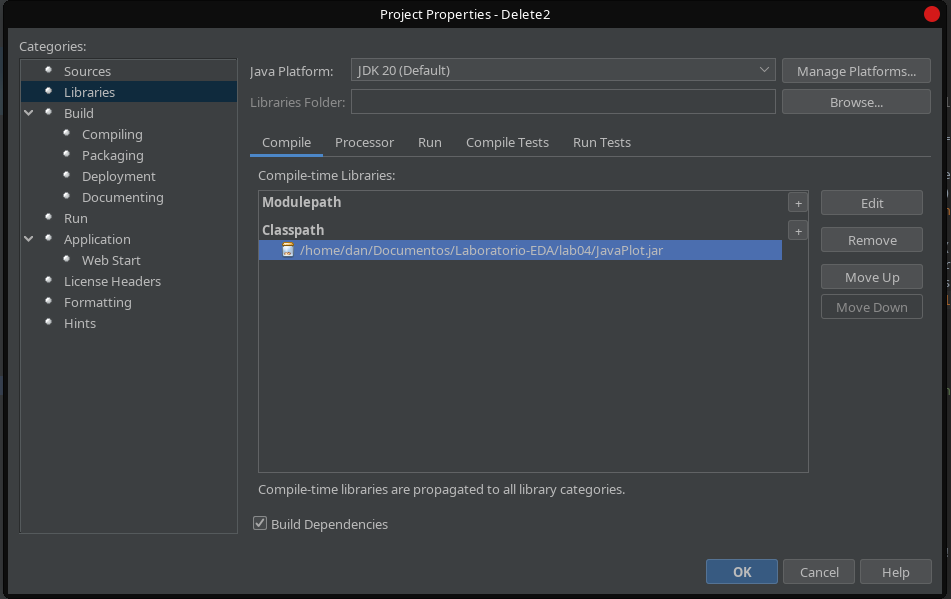
\includegraphics[scale=0.4]{img/net.png}
		\end{center}
	\end{figure}
	
	\begin{itemize}
		\item Si queremos correrlo desde terminal, por ejemplo, ubicandonos en el ejercicio 2 debemos especificar el classpath al momento de compilarlo y ejecutarlo de la siguiente forma, (No olvidar que en este caso el .jar es \verb|JavaPlot.jar|).
		
		\begin{lstlisting}[language=bash, caption={caption}][H]
			Laboratorio EDA:(main) $
			Laboratorio EDA:(main) $ javac -cp lab04/JavaPlot.jar *.java
			Laboratorio EDA:(main) $ java -cp lab04/JavaPlot.jar:. Test
		\end{lstlisting}
	\end{itemize}
	
\end{itemize}